%
% PENSER À :
% - vérifier taille de police et interligne
%

\documentclass[a4paper,12pt]{report}

\usepackage[utf8]{inputenc}
\usepackage[T1]{fontenc}
\usepackage[francais]{babel}

\usepackage[a4paper,top=3cm,bottom=3cm]{geometry}

\usepackage{graphicx}
\usepackage{pdfpages}

\usepackage{fancyhdr}
\pagestyle{fancy}
\renewcommand\headrulewidth{1pt}
\rhead{ \LaTeX }
\cfoot{ \thepage }

\usepackage{titlesec}

\titleformat{\chapter}{\normalfont\huge}{\thechapter.}{20pt}{\huge}

\renewcommand{\chaptername}{ }
\DeclareTextFontCommand{\emph}{\bfseries}

\newcommand{\para}[1]{\par{#1}\\}

\title{QBITS}
\author{QUÉLARD Xavier}
\date{ \today{} }

\makeindex

\begin{document}

%
% -----------------------
% [1] PAGE DE GARDE
% -----------------------
%

%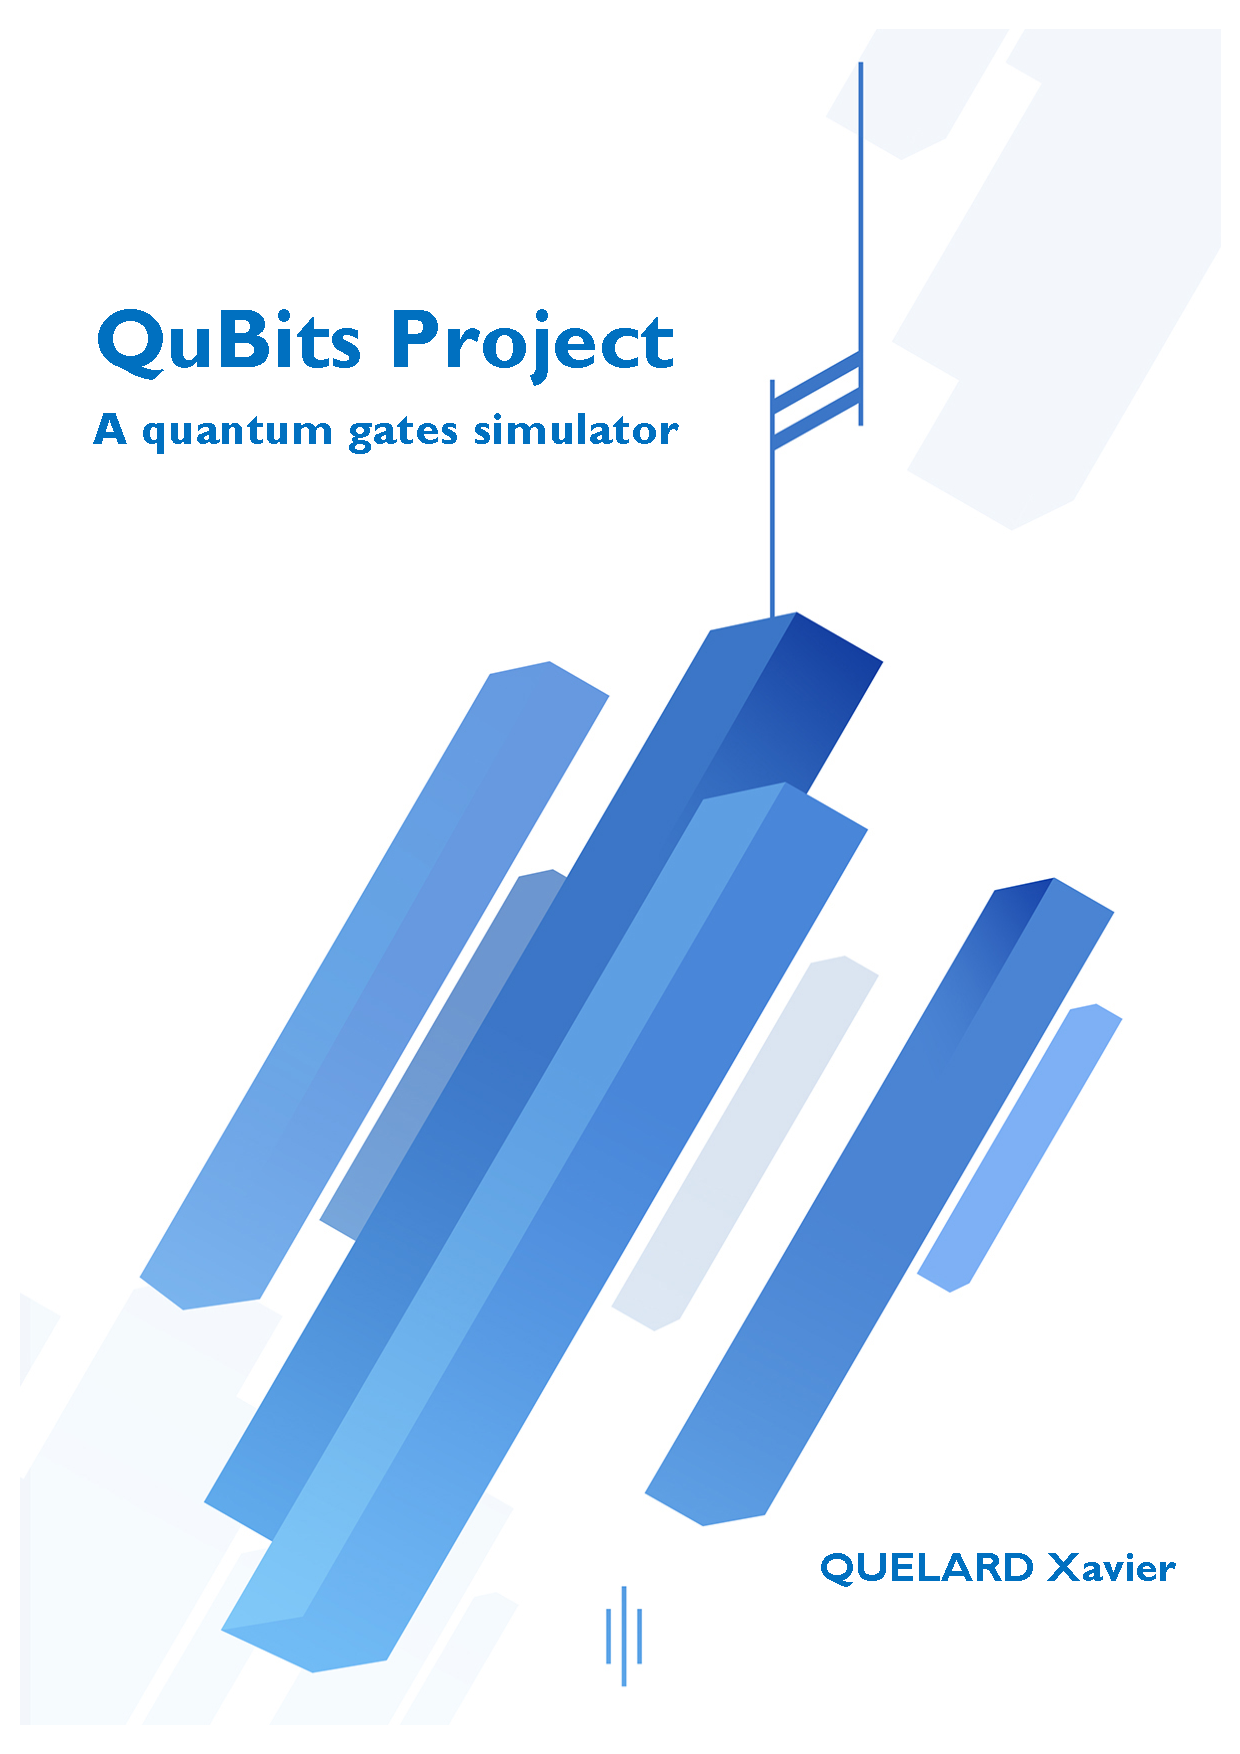
\includepdf{Garde}
\maketitle

%
% -----------------------
% [2.5] ABSTRACT
% -----------------------
%

\chapter*{Résumé}

\para{
	...
}

%
% -----------------------
% [2] REMERCIEMENTS
% -----------------------
%

%
% -----------------------
% [3] TABLE DES MATIERES
% -----------------------
%

\tableofcontents

%
% -----------------------
% [4] INTRODUCTION
% -----------------------
%

\chapter*{Introduction}
\addcontentsline{toc}{chapter}{Introduction}

\para{
	...
}

\chapter{Chapter1}

%
% -------------------------
% [5] I -> CONTEXTE DU JOB
% -------------------------
%

	\section{section1}

\para{
	...
}

	\section{section2}

\para{
	...
}

%
% -----------------------
% [?] CONCLUSION
% -----------------------
%

% PARLER DE L'APRENTISSAGE DE LATEX ET GITHUB!

\chapter*{Conclusion}
\addcontentsline{toc}{chapter}{Conclusion}

\para{
	...
}

\chapter*{Bibliographie}

\para{
	...
}


\chapter*{Annexe}

\end{document}
